\documentclass[a4paper, 10pt]{article}
\usepackage[UTF8]{ctex}
\usepackage{geometry}
\usepackage{indentfirst}
\usepackage{amsmath}
\usepackage{amssymb}
\usepackage{graphicx}
\usepackage{subfigure}
\usepackage{enumerate}
\usepackage{listings}
\usepackage{appendix}
\usepackage{xcolor}
% \usepackage[table,xcdraw]{xcolor}
\usepackage{multirow}
\usepackage{algorithm}
\usepackage{algorithmicx}
\usepackage{algpseudocode}
\usepackage{amsmath}
\renewcommand{\algorithmicrequire}{\textbf{Input:}}
\renewcommand{\algorithmicensure}{\textbf{Output:}}
\lstset{
    numbers=left,
    numberstyle= \tiny,
    keywordstyle= \color{ blue!70},
    commentstyle= \color{red!50!green!50!blue!50},
    frame=shadowbox,
    rulesepcolor= \color{ red!20!green!20!blue!20} ,
    escapeinside=``,
    xleftmargin=1em,xrightmargin=0em, aboveskip=1em,
    framexleftmargin=2em,
    showstringspaces=false,
    showtabs=false,
    breaklines=true
}

\title{Report of Final Project}
\author{Wang ZhongYe}

\begin{document}

\maketitle

\section{成果展示}
我们的搜索引擎采用Bootstrap作为前端的框架,利用Javascript实现了与模型有关的部分的前后端的异步交互,避免页面的加载时间过长。我们的搜索引擎后端利用web.py实现对网页前端的支持,使用高效的elastic-search实现数据的索引和搜索。

我们使用额外数据和词频分析建立了现代诗和古诗的词典和TF-IDF词典,并借助jieba的有关功能实现了现代诗和古诗文的文本分析和关键词抽取。我们使用深度卷积神经网络实现了图片到物象的转化以及建立图片与诗歌间的联系从而实现为诗歌配图、由图片搜索和生成现代诗和古诗文。

\paragraph*{首页推荐} 图\ref{fig:demo_landing}所示为我们搜索引擎的首页,其中包含了每日自动更新的推荐内容,和每次刷新都会更新的诗歌推荐内容。推荐的具体算法可以通过浏览器的Cookie取回用户的常用搜索关键词进行相似度推荐,或利用用户浏览的诗歌进行关联推荐。由于时间原因,我们未能着手实现推荐算法,目前使用随即取回诗歌填充推荐的内容。

\begin{figure}[H]
\centering
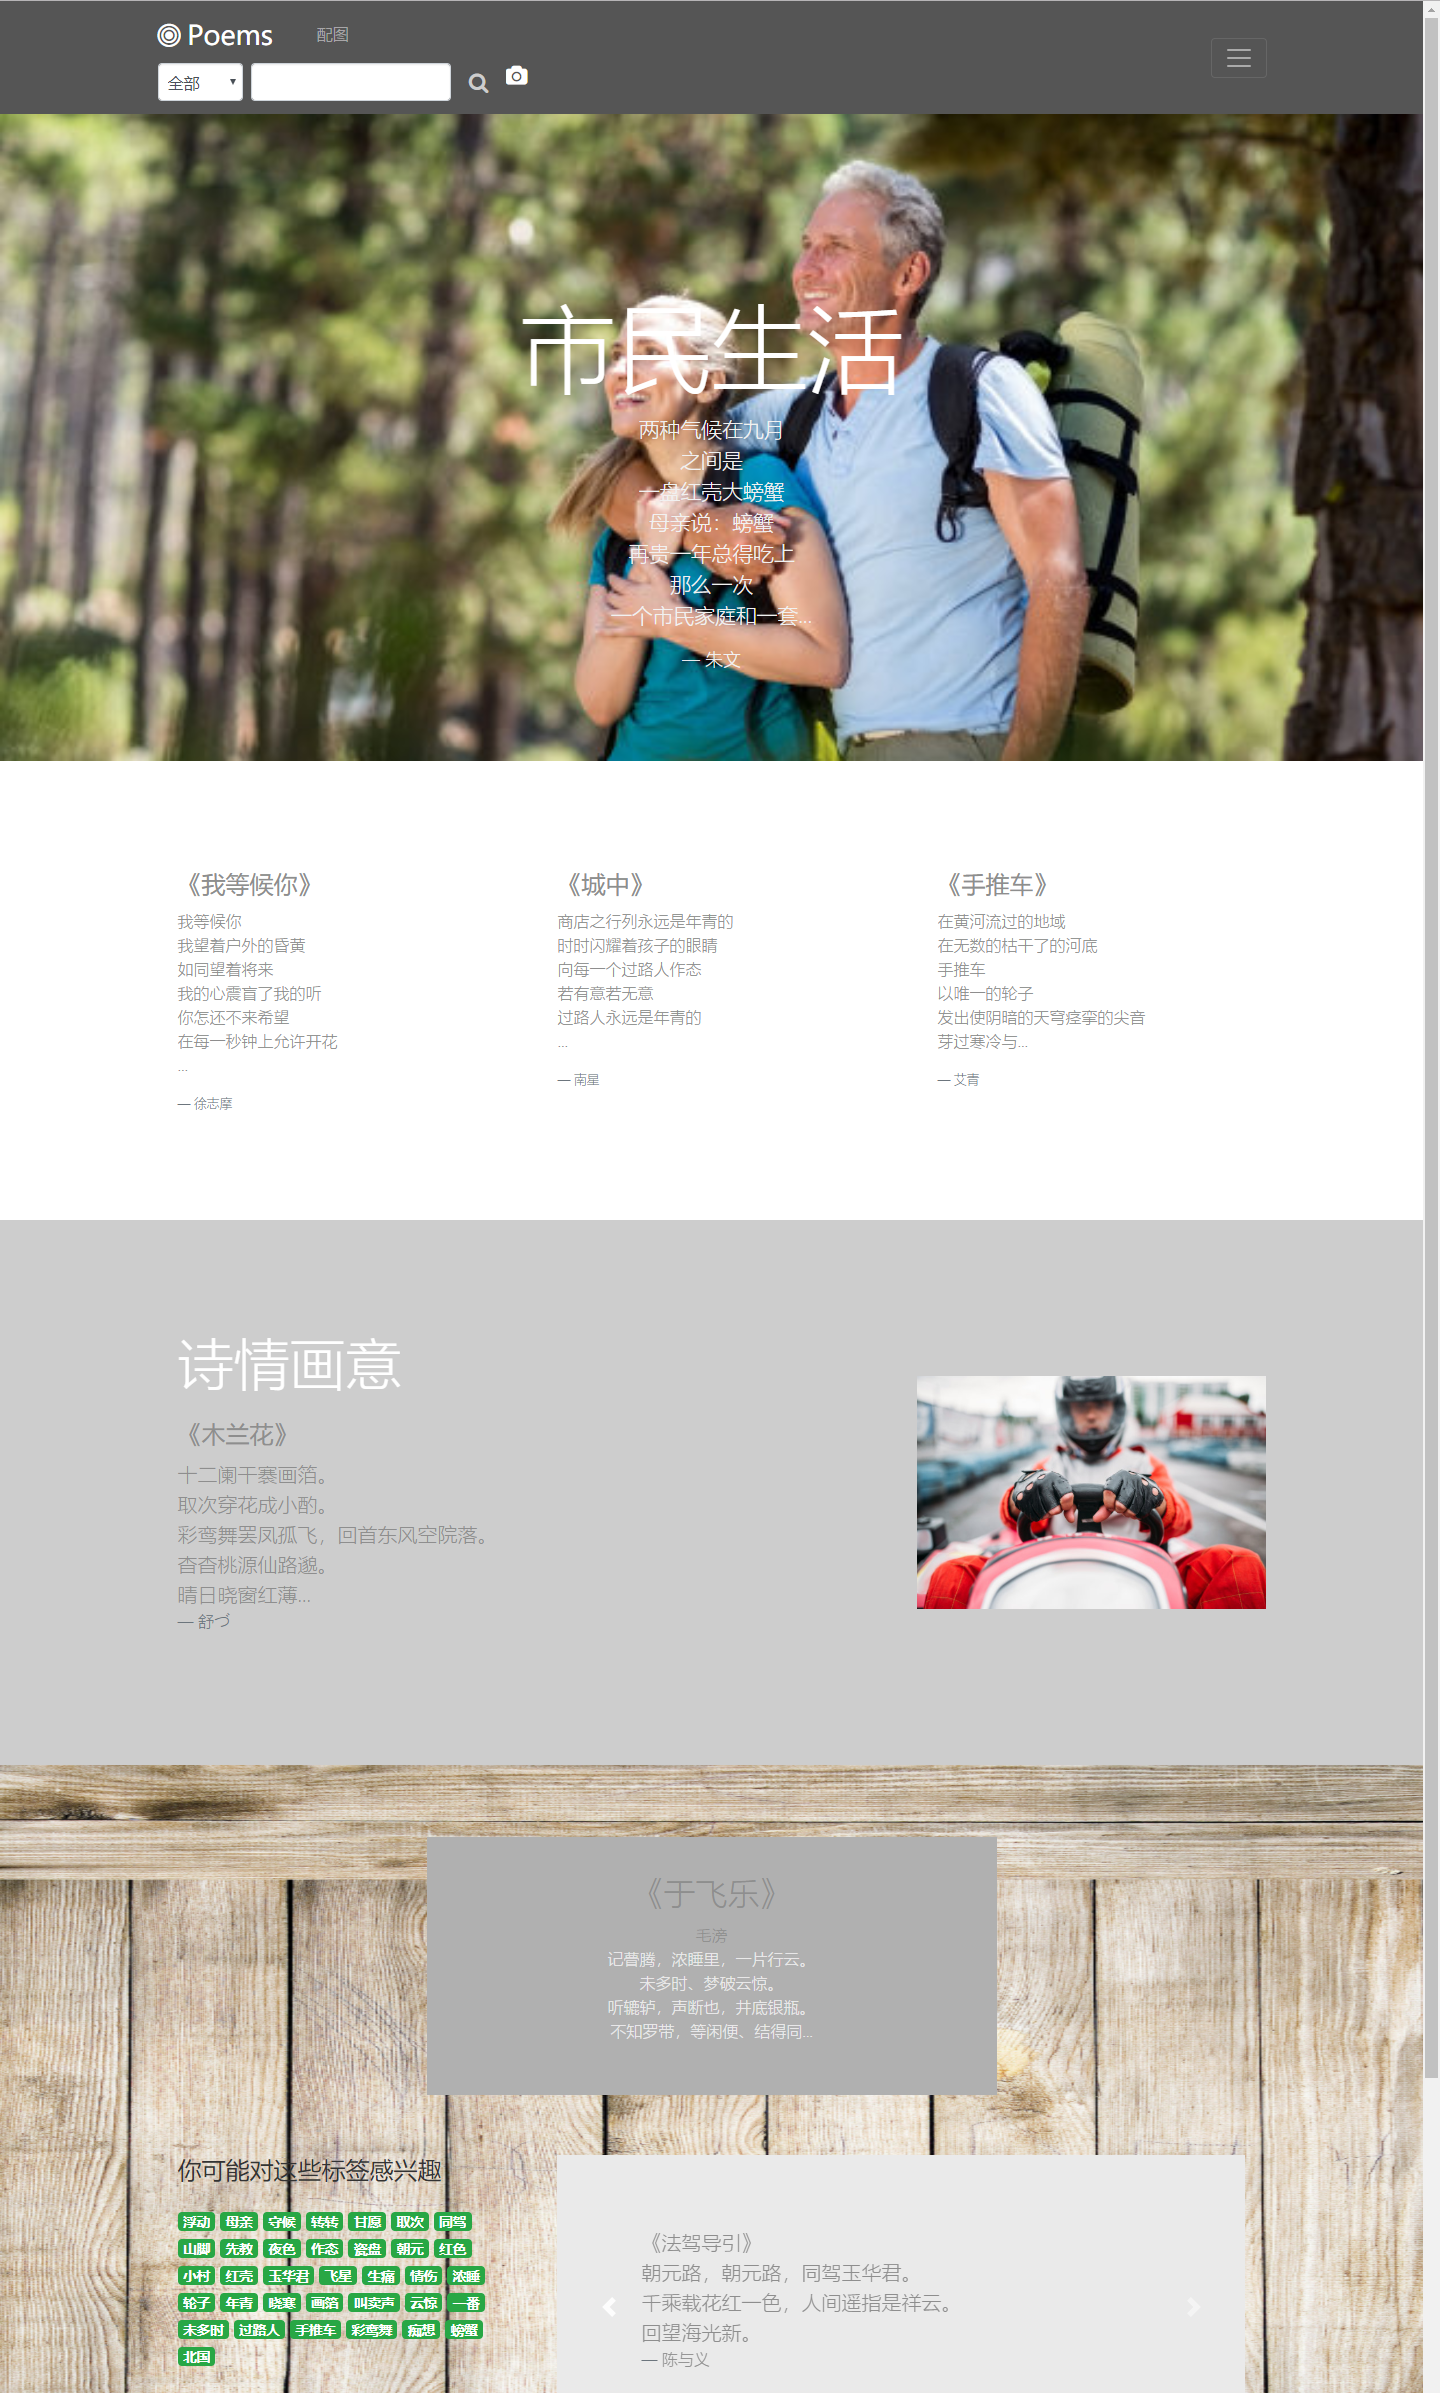
\includegraphics[scale=0.45]{fig/demo_landing.png}
\caption{网站首页}
\label{fig:demo_landing}
\end{figure}

\paragraph*{搜索接口} 作为一个搜索引擎,其最核心的页面要素便是搜索接口。图\ref{fig:demo_searchbar}所示为我们搜索引擎提供给用户的接口,该接口在网页所有页面都存在。该搜索表单嵌入在页面的导航栏中,默认情况下收起高级搜索表单,仅显示搜索诗歌的类型(全部、现代诗、古诗文)和模糊搜索输入框,展开后用户可以自定义当前的查询细节。

\begin{figure}[H]
\centering
\includegraphics[scale=0.5]{fig/demo_searchbar.png}
\caption{搜索接口}
\label{fig:demo_searchbar}
\end{figure}

首先,我们允许用户选择在哪些域中进行模糊搜索。打开相应的开关可以另当前查询包括相应的域,有多个域被选择后,搜索引擎将返回匹配尽可能多的域的结果。翻译和赏析仅对古诗文搜索类型有效。如果所有域都被关闭,当前查询会被归类为无效查询并反馈相应信息给用户。网页默认开启所有的搜索域。

其次,我们提供同义词扩展功能。当用户对查询的关键词不确定时,可以开启这一功能,搜索引擎将会利用内置的词库对查询中的每个词进行同义词扩展,扩大搜索结果的覆盖范围,提高用户找到所希望得到的结果。这一功能仅对在内容中搜索的查询进行扩展。

最后,我们提供精确查询接口,让用户进一步明确当前查询的细节。对于不同的查询类型,我们提供不同的搜索域。对于古诗文,用户可以明确诗歌的标题、作者、标签、朝代或类型(诗、词、曲等);对于现代诗,用户可以明确诗歌的标题、作者、标签、流派或年代。如果一个域在精确搜索中被使用,该域中的搜索将不会使用模糊搜索框中的字段。

图\ref{fig:demo_searchbar}中所示的样例查询仅在作者域中模糊搜索“李白”这一字段,不使用同义词扩展,在标题域中精确搜索“静夜思”这一字段。其余字段为空将不对它们进行精确搜索。

除此之外,用户还可点击搜索按钮边上的相机按钮,上传希望分析并用于搜索诗歌的图片。用户还可通过上方的链接跳转至配图页面,上传自创的诗歌并为之匹配合适的图片。


\paragraph*{结果页面} 图\ref{fig:demo_accres}所示为上述查询的搜索结果,可见搜索引擎精确的返回了一条作者是李白,诗名为《静夜思》的诗歌。

\begin{figure}[H]
\centering
\includegraphics[scale=0.48]{fig/demo_accres.png}
\caption{精确搜索结果}
\label{fig:demo_accres}
\end{figure}

点击单首诗歌可以跳转到如图\ref{fig:demo_poempage}所示的相应的诗歌内容页面。该页面会显示诗歌的完整内容、标签以及相应配图。

\begin{figure}[H]
\centering
\includegraphics[scale=0.48]{fig/demo_poempage.png}
\caption{单首诗歌内容页面}
\label{fig:demo_poempage}
\end{figure}

如果解除精确搜索,并在所有域中模糊搜索“李白”这一字段,将返回如图\ref{fig:demo_vagueres}所示的结果页面。其中显示该查询共有136条匹配结果,并且每页显示一定数量的结果诗歌。

\begin{figure}[H]
\centering
\includegraphics[scale=0.475]{fig/demo_vagueres.png}
\caption{模糊搜索结果}
\label{fig:demo_vagueres}
\end{figure}

对于每首诗歌,我们通过??为其匹配了一张图片,并通过诗歌文本分析的算法结合先前爬取的数据对其添加合适的标签,同诗歌一起展示给用户。如果诗歌长度过长,将会截断一定长度后显示。在电脑浏览器上看,每条结果的大小参差不齐,但我们是针对手机端开发的网站,在手机端上浏览效果比较好。由于结果数目较多,我们实现了搜索结果的分页显示。

用户也可以浏览单个作者的信息及其所有作品,该页面同搜索结果页面采用相同的实现形式和页面效果,再次不再作图片展示。


\paragraph*{诗图转换} 除了文本搜索,我们还实现了图片与诗歌间的转化。图\ref{fig:demo_analyze}所示为图像分析页面,这里显示了对用户上传的图片的分析结果,用户可以在分析结果的基础上进一步搜索诗歌或者生成诗歌。图中是现代诗生成结果的样例。

\begin{figure}[H]
\centering
\includegraphics[scale=0.48]{fig/demo_analyze.png}
\caption{图像分析页面}
\label{fig:demo_analyze}
\end{figure}

图\ref{fig:demo_matchimage}是诗歌配图页面的样例。这里,用户可以上传自己创作的诗歌,并为这首诗歌匹配图片。图中以“青草在奔跑”为例进行配图,结果中以奔跑为主题的图片居多。

\begin{figure}[H]
\centering
\includegraphics[scale=0.48]{fig/demo_matchimage.png}
\caption{诗歌配图页面}
\label{fig:demo_matchimage}
\end{figure}

以上便是我们搜索引擎的简要的展示,接下来我们会详细介绍各部分的实现细节。

\section{后端实现}
在这一部分,我们将介绍搜索引擎的后端实现,包括网站的后端实现和数据库搜索的实现。

\subsection{网站架构}
\begin{figure}[H]
\centering
\includegraphics[scale=0.48]{fig/web_struct.png}
\caption{网站架构}
\label{fig:web_struct}
\end{figure}

图\ref{fig:web_struct}是我们搜索引擎的网站架构。

我们的网站采用了一定的MVC分离。PoemSeachES和netModel及model文件夹下的模型为搜索引擎的模型部分,负责对controller发出的查询请求做出响应和进行图像处理。controller.py为我们的控制器,图中由淡蓝色矩形框出的类都有对应的前端页面,深蓝色标出的三个类通过前端的javascript进行动态加载,异步返回数据。static是web.py框架下网站的资源文件夹,其中的js文件夹和css文件夹包含了支持前端布局的js文件和css文件,其余三个文件夹用于缓存用户上传和图像处理中间结果的图片。

\begin{table}[H]
\centering
\begin{tabular}{ccc}
\hline
\textbf{类} & \textbf{URL} & \textbf{页面} \\ \hline
index & /index & 首页推荐 \\
query & /query & 文本和图像查询处理结果页面,无翻页功能 \\ 
gallery & /gallery & 同query,但只处理文本查询,提供翻页接口 \\ 
poempage & /poempage & 单首诗歌内容页面 \\ 
authorpage & /authorpage & 单个作者信息及作品页面,类似gallery \\ 
matchimage & /matchimage & 诗歌配图页面 \\ 
analyzed & /analyzed & 图像分析页面 \\ 
notfound & /notfound & 404页面 \\ \hline
\end{tabular}
\caption{链接对应关系}
\label{tab:url_connect}
\end{table}

controller中各个类对应的url及前端页面功能如表\ref{tab:url_connect}所示。

在controller.py中,我们还有一系列辅助函数存放在validator类下,用来进行表单验证和表格输入的预处理。其中最主要的两个函数是form\_validate和to\_command\_dict。

form\_validate对于用户通过表单的输入进行验证并返回验证结果供调用者进一步判断页面的跳转。该函数会判断用户的输入是否为空,其会检查所有可能成为有效输入的域,包括高级搜索中的精确搜索域。该函数还会检查表单输入的合法性,来避免用户的恶意访问。两个关键的准则是表单中包含searchType和query这两个域,因为他们确定了查询的索引和查询的内容(虽然query可以为空),和存在query模糊查询时高级搜索中的搜索域选择非空,否则这条查询无法转化成模型可以处理的命令。对于其他只应该由我们规定的内链所引起的查询,我们或者重用了form\_validate,或者实现了各自的验证函数来保证没有会造成严重后果的恶意访问发生。

to\_command\_dict根据表单提供的不同的查询约束,生成对应的查询域和查询值的映射并规定每一条约束是否为强制的(精确查询的)。这个函数的意义在于实现搜索引擎建立与数据库建立、控制器与模型的解耦,避免了在多个文件中修改关键字名称的工作。

\subsection{索引搜索}

\subsubsection{文本搜索}
首先,我们将介绍我们是如何利用elastic-search实现基于文本的诗歌搜索的。



\end{document}